\documentclass[sigplan,anonymous,review]{acmart}

\usepackage{authorcomments}
\usepackage{listings}
\usepackage{algorithm}
\usepackage{algpseudocode}
\usepackage{xspace}
\usepackage{paralist}


\lstset{language=R}
\definecolor{LightGray}{rgb}{.92,.92,.92}
\definecolor{Gray}{rgb}{.3,.3,.3}
\definecolor{DarkGray}{rgb}{.5,.5,.5}
\lstset{ %
  columns=flexible,
  captionpos=b,
  frame=single,
  framerule=0pt,
  tabsize=2,
  belowskip=0.5em,
  backgroundcolor=\color{LightGray},
  basicstyle=\small\ttfamily,
  emphstyle=,
  keywordstyle=,
  commentstyle=\color{Gray}\em,
  stringstyle=\color{Gray},
  numbers=left,
  showstringspaces=false
}
\lstdefinestyle{R}{ %
  language=R,
  morekeywords={assign, delayedAssign},
  deletekeywords={env, equal, c, runif, trace, args, exp, t, all},
  breaklines=true
}
\lstdefinestyle{Rin}{ %
  style=R,
  breaklines=false
}


\newcommand{\tool}{\texttt{signatr}\xspace}
\newcommand{\numFnsCaseStudy}{20\xspace}
\newcommand{\numPkgsScaleStudy}{20\xspace}
\newcommand{\code}[1]{{\lstinline[style=Rin]!#1!}\xspace}

% For algorithmcx
\algnewcommand{\LineComment}[1]{\State \(\triangleright\) #1}

\begin{document}

\title{\tool Fuzz Your Trace Typing}

\begin{abstract}
The abstract will go here.
It will be great.
The greatest abstract.

\end{abstract}

\maketitle

I set up author comments for everyone: \AT{for Alexi}, \PB{for Pierre}, \FK{for
Filip}, and \JV{for Jan}, oh and \TODO{for TODOs}. Feel free to change the
colours in {\tt authorcomments.sty}.

\FK{ 
Plan: 
- Abstract + Introduction + R background (1.5 page)
- Approach (2.25 pages)
    - overview of the approach
    - details about the components
    - a figure how it fits together
        - show the two pipelines in one figure highlighting the individual packages
- Experiment (1 page)
    - questions:
        - Are traces enough?
        - How polymorphic are polymorphic functions?
    - setup: machine, corpus size, ...
    - result: a table with number of type signatures for base arithms and use packages
- Conclusions (.25 page)
- Appendix
  - show code listings from the various steps of the pipeline
}


\section{Introduction}
\label{sec:introduction}

% Retrofitting type systems onto dynamic languages is desirable.
% __ helps reasoning about code
% __ helps maintainability
Dynamic languages are ubiquitous.
For example, JavaScript is the most popular language on GitHub (according to the state of the Octoverse~\cite{state-of-octoverse-2021}), and is the lingua franca of web development both client-side, and server-side thanks to Node.js.
Python is the next most popular language on GitHub, owing a lot of its popularity to its use in the machine learning community.
For nontraditional programmers such as scientists and statisticians, R is often the language of choice for their statistical analyses.
The ease of use of these languages plays a big part in their popularity, as many new programmers gravitate to them for their unobtrusive semantics.
That said, dynamic languages are notoriously difficult to reason about statically (\AT{cite some stuff here}), as the dynamism inherent in the semantics complicates static analyses.

% There are a few type systems for dynamic languages.
% __ TypeScript, etc.
To help curtail language dynamism, significant effort has been expended in retrofitting static type systems onto these languages; this is known as \textit{gradual typing}.
In a gradually typed program, typed and untyped code can coexist, and the precise flavor of the gradual type system dictates how typed and untyped code interact: for instance, types can be checked and enforced at runtime in sound gradual typing (in languages such as SafeTypeScript~\cite{rastogi2015safe}), or entirely ignored in optional gradual typing (e.g., in TypeScript).
As it happens, TypeScript is the fourth most popular language in the aforementioned state of the Octoverse~\cite{state-of-octoverse-2021}, and the added static types help projects evolve with grace with their added documentation.

% Retrofitting type systems onto dynamic languages is complicated.
% __ highly dynamic features can be hard to describe statically, and can be expensive to check
% __ language semantics are sussy
Designing a useful gradual type system for a dynamic language is difficult as dynamism is pervasive in these languages, and describing highly dynamic code statically is fraught.
For example, the \code{eval} function that executes arbitrary strings as code is frequently used in JavaScript~\cite{richards2011eval}, and reasoning about what that code does ahead-of-time is extremely challenging.
TypeScript, along with all other gradually typed languages, includes an \code{any} type for these situations, which essentially states that no information about the value is known.
This \code{any} type is essentially an ``escape hatch'' that lets programmers escape the type system when they want to do something dynamic, and designing a type system that minimizes the need for said escape hatch is desirable; to that end, gradual type system designers should be aware of how the language is used in practice, and e.g. recent work~\cite{turcotte2020designing} reports on a large corpus analysis of R code in an effort to understand how programmers use the language, and authors leverage this information to design a simple type annotation language for R functions.
\AT{More examples? Maybe trace typing.}

% Beyond accounting for existing code, we must account for other, unexpected inputs.
% __ as compared with trace typing
% __ type systems must guard against new inputs
\AT{I think there's a subtle argument to be made here. 
It's not enough to look at existing code, because really your type system does two things: a type on a function describes what your function accepts, and, implicitly, \textit{also what it rejects}.
In that sense, fuzzing can be an important part of inferring a type for something.}
Focusing on designing type systems that account for existing code is a good start, but inevitably new code will be written that an effective type system must deal with.
In a sense, static types on function parameters help guard a function against unexpected inputs, and so it is important when evaluating potential type systems to exercise code in unexpected ways. 
For example, a programmer might not be aware that their code can be exercised in a certain way, and existing code has not fully exercised the function (e.g., perhaps the programmer did not fully test their function).

% Fuzzing to the rescue?
Fuzzing is a technique wherein functions are called with many inputs to try to find bugs.
This technique could be leveraged to instead try to find successful calls to a function.
The resulting approach can be used by type system designers to see how their types match up with possible function use, rather than just intended function use.
Moreover, it could be used by developers to help infer specifications for their functions, and help them understand how their code behaves in the wild.

% We propose an approach for evaluating type system designs against both existing and new code.
% __ trace collects existing calls and values
% __ database indexes values, provides query API
% __ fuzzer takes advantage of massive amounts of realistic inputs to generate new function inputs
% __ merge strategy parameterized over type systems T expressed as (1) a function to determine the type of a value, and (2) a set of rules describing which pairs of types are compatible
% __ large scale evaluation of type system designs for R
In this work, we propose an approach for evaluating gradual type system designs with respect to both existing and new code.
We develop a tracer that collects information about function calls and values observed during code execution.
This information, and in particular the values observed during execution, are stored in a database with an expressive query API.
We propose a fuzzing approach that relies on this database to generate new function inputs based on massive amounts of existing observed values.
Finally, we develop an approach for synthesizing the results of fuzzing into a type signature for a function, entirely parameterized over a type system expressed as (1) a function to infer the type of a value, and (2) a function to determine if one type is a subtype of another.

In summary, the contributions of this paper are:
%
\begin{inparaenum}[(1)]
    \item a new approach to trace typing which adds fuzzing based on database of real, complex values, and
    \item an implementation of this approach in a tool called \tool for the R programming language.
\end{inparaenum} 
Using the tool, we generate a value database \TODO{DB stats} and use it to fuzz trace types for \TODO{experiment stats}.
We find \TODO{result stats}.
%
The tool is open source and including the dataset used for this paper, it is available online.

\paragraph{The R Programming Language}

R sports an unusual mix of language features making it a challenging target for
tooling~\cite{morandat2012evaluating}. The relevant features are the following:

\FK{It should be relevant for building the tool right?}

\begin{compactitem}[$-$]

\item R does not have type annotations or a static type system. This means
    there is nothing to suggest what the expected arguments or return values of
    a function could be, and thus there is little to guide test generation.

\item Most values are vectors or lists. Values can be annotated by key-value
    pairs called attributes. These annotations, coupled with reflection, are
    the basic building blocks for many advanced features of R. For example, the
    S3 dynamic dispatch mechanism (in fact R has multiple different object
    systems but S3 is the most widespread one) is based on these attributes. An
    R object is simply a value with \code{class} attribute denoting the class
    the object is \texttt{instance-of}.

\item Built-in types are automatically and silently coerced from more specific
    types to more general types when deemed appropriate. There are no global
    coertion rules, instead, each function does the coertion of its parameters
    as it finds it fit.

\item All expressions are evaluated by-need, thus the call \code{f(a+b)}
    contains three delayed sub-expressions, one for each variable and one for
    the call to plus. This means that R does not pass values to functions but
    rather passes unevaluated promises (the order of evaluation of promises is
    part of the semantics as they can have side effects). These promises can
    also be turned back into code by reflection.

\item R has a copy-on-write semantics for shared values. A value is shared if
    it is accessible from more than one variable. This means that side effects
    that change shared values are rare. This gives a functional flavor to large
    parts of R.

\item The primary abstraction in R is a function. Functions are grouped into
    packages that can be imported. A function can be generic, allowing an
    object-oriented style of programming. \TODO{Some stats about how many
    parameters R functions have.} 

\end{compactitem}

\FK{Typer paper gave us a foundation for an eventual type system for R.
It was trying to answer the quetions about:
(1) What expressive power is needed to accurately type R code? 
(2) Which type system is the R community willing to adopt?
In this paper we want to move one step closer to the actual type system.
Some questions:
(1) Are the traces we used before enough? The reason for this question is that one of the key point of dynamic languages is that they try to "fail" as little as possible - they keep going even if the shape of the data is not exactly what it should be. So the question is what all a function can take and ideally what still makes sense (though this is much harder to get without oracles),
(2) How polymorphic are the polymorphic functions that we see?
(3) What should be the type base functions?
(4) How about S3 dispatch and coertion?
}


\FK{Few things to mention (random notes): (1) we are looking at type systems for users (not machines), e.g. a user would likely prefer an arrow of union while a compiler would do better with a union of arrows.
(2) R is somewhat different from Python and JS in the way that it lacks any sort of modules (modulo S4,...). In JS/Python we have classes and objects in the OOP style - that is not what we have in R - or at least not in the same sense. The S3 generics are tricky because they encapsulate too many different objects - it is really an adhoc polymorphims, much like operation overloading. (4) This is second paper in the series of papers whose goal is to design a type system for R. In the first one we used the trace-typing technique to gather data that can be fed into the design process. This one goes one step further and extend the search space to get more accurate function specification. (3) Inferring subtyping is hard - example with data.frame / tibble how one can get it wrong.
}

\section{Related Work}
\label{sec:background}

\FK{The typer paper should be mentioned in introduction so what shall be here? The tracing types paper~\cite{andreasen2016trace}, randoom?, quickcheck?, genthat?}

% \subsection{The R Programming Language}
%
% \AT{We can probably illustrate many of the issues we grapple with in this section, which will help the reader understand R, as well as the slew of issues we face while fuzzing.}
%
% % Introduction to R.
% R is one of the most popular data science languages, and sports an unusual mix of language features~\cite{morandat2012evaluating}: it is a vectorized, lazy, dynamic, functional, object-oriented programming language.
% As an appetizer, consider the following simple R script:
% \begin{lstlisting}[escapechar=|]
% x <- 1|\label{code:basic-assign-start}|
% y <- c(2, 3)
% z <- c(4, 5, 6, 7)|\label{code:basic-assign-end}|
%
% x + y # ==> c(3, 4)|\label{code:basic-scalar-vector-add}|
% y + z # ==> c(6, 8, 8, 10)|\label{code:basic-vector-vector-add}|
% \end{lstlisting}
% Here, lines~\ref{code:basic-assign-start}-\ref{code:basic-assign-end} assign \code{1} to the variable \code{x}, and vectors \code{[2, 3]} and \code{[4, 5, 6, 7]} to \code{y} and \code{z} respectively (note: \code{c} is the vector constructor in R).
% As it happens, what appears to be the scalar \code{1} is actually a unit-length vector containing \code{1}, and R does not distinguish between the two (e.g., \code{1 == c(1)}).
% Line~\ref{code:basic-scalar-vector-add} adds \code{1} to each element of the vector \code{c(2, 3)}, and line~\ref{code:basic-vector-vector-add} shows how vectors of different lengths can be added with the same \code{`+`} function (here, the 2 length vector is duplicated and added to the longer one).
% These vectors are homogeneous in that they can only contain values of a given primitive type.
% \AT{Probably a little more to say about this.}
%
% % Types.
% R has a few notions of type, and the two most commonly used are the \textit{type tag} of a value \code{v}, accessed through \code{typeof(v)}, and the \textit{class} of \code{v}, accessed through \code{class(v)}.
% The \code{typeof} type of a value cannot be changed, and includes six primitive types (logical, integer, double, complex, character, and raw byte), a list type, an environment type, and many more.
% The class of a value can be changed easily at run time by assigning to a value's class attribute (e.g., \code{class(x) <- "SomeNewClass"}), and the class of a value is nothing more than a list of class names.
%
% % Dispatch.
% The class of values is important at run time as R has dynamic dispatch mechanisms (in fact, R has many different dynamic dispatch mechanisms, but we focus on the most widespread S3 single dispatch in this paper). 
% In S3 dispatch, functions can be declared to dispatch on the class of a value.
% Consider:
% \begin{lstlisting}[escapechar=|]
% foo <- function(x) { UseMethod("foo", x) }|\label{code:dispatch-generic}|
% foo.A <- function(x) { "you called foo.A" }|\label{code:dispatch-A}|
% foo.B <- function(x) { "you called foo.B" }|\label{code:dispatch-B}|
%
% q <- 2
% class(q) <- "A"
% foo(q) # ==> "you called foo.A"|\label{code:dispatch-call-A}|
% class(q) <- "B"
% foo(q) # ==> "you called foo.B"|\label{code:dispatch-call-B}|
% \end{lstlisting}
% On line~\ref{code:dispatch-generic} a function \code{foo} is defined to dispatch on the class of parameter \code{x} through \code{UseMethod("foo", x)}, which essentially states that \code{foo.CN} will be called if \code{class(x) == "CN"}.
% This is evidenced on line~\ref{code:dispatch-call-A}, where \code{foo.A} is called since \code{class(q)} is \code{"A"}, and similarly on line~\ref{code:dispatch-call-B} with \code{q} having changed to class \code{"B"}.
%
% % Problems with dispatch
% Dynamic dispatch, dynamic typing, and the class of values being so fluid contribute heavily to the unpredictability of R code.
% Any S3 dispatch method (like \code{foo} in the previous code snippet) can be extended with more dispatch targets dynamically by defining new functions at run time (e.g., defining other \code{foo.CN}).
% \AT{Ugh, reword:} This, combined with the fact that the class of a value is ignored by R unless it is needed, means that the behavior of a function may change unexpectedly as new classes and dispatch targets are introduced.

\emph{Randoop}~\cite{pacheco2007randoop} is a feedback-driven random test generation tool for Java, though the technique underpinning it is universally applicable; \AT{in fact, we implemented a version of this technique in R as the baseline for our evaluation}.
The technique described in the \emph{Randoop} paper generates sequences of method calls to test classes, and randomly generates arguments for these calls in two ways: for primitives, a random value is selected from a predefined, but user-extensible list, and for reference types a value is selected at random from those which have been seen, and if none are available then {\tt null} is selected.
This technique is effective at generating tests involving non-trivial objects that are built up from a number of method calls, but these are uncommon in data science languages.

\AT{Add quickcheck}

\subsection{Test Generation for Dynamic Languages}

Many of the aforementioned techniques rely on static function parameter types in creating values with which to call a function, and dynamic languages do not have static type information.
For example, \emph{LambdaTester}~\cite{lambdatester} focuses on test generation for higher-order functions in JavaScript; a discovery phase is required to identify which parameters are expected to be callbacks, and all other, non-callback arguments are generated in a similar manner to \emph{Randoop}.
Further work on \emph{Nessie}~\cite{arteca2022nessie} expanded upon the approach presented in \emph{LambdaTester} to generate tests for asynchronous callbacks using sequencing and nesting.
Other work on fuzzing deep-learning libraries in Python~\cite{wei2022free} explicitly cite Python being a dynamic language as a challenge for test generation; an important part of the pipeline in the paper is inferring types for function parameters by running existing code.

\AT{A few disparate things on Python, Alexi has the links.}

\section{Fuzzy Trace Typing}
\label{sec:fuzzy}

\subsection{Overview}

\begin{itemize}
    \item We built a tracer and ran it on a bunch of R code, observing values and their origins. 
    %
    \item The information obtained via tracing is collected in a database equipped with a rich query API. 
    The origins of values can be used reconstruct the calls (in the same manner as previous work~\cite{turcotte2020designing}), and the database of values can be queried to find other potential inputs to functions.
    %
    \item We developed a fuzzer called \tool that takes advantage of this database to construct additional calls with \textit{realistic data} to further exercise functions.
    %
    \item Finally, a data analysis pipeline processes the output of the fuzzer to prepare static type signatures for fuzzed functions.
\end{itemize}

\begin{figure}
    \centering
    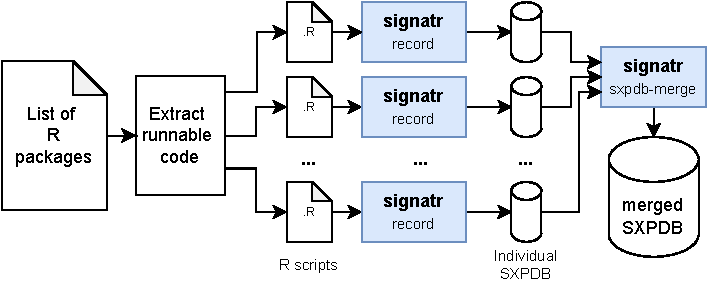
\includegraphics[width=\columnwidth]{code-and-figures/sxdb-pipeline.pdf}
    \caption{SXPDB creation pipeline}\label{fig:sxpdb-pipeline}
\end{figure}

\begin{figure}
    \centering
    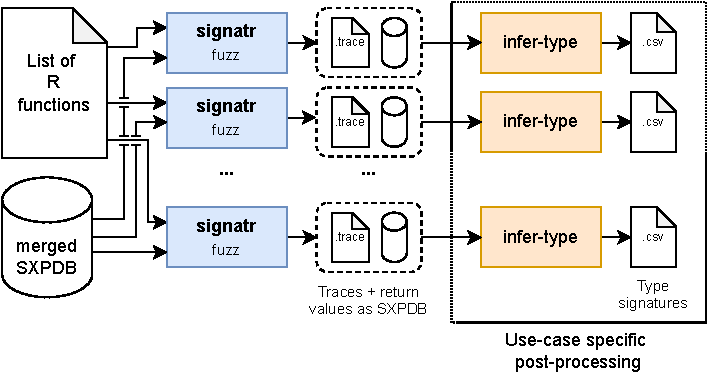
\includegraphics[width=\columnwidth]{code-and-figures/fuzz-pipeline.pdf}
    \caption{Fuzzing pipeline}\label{fig:fuzz-pipeline}
\end{figure}

\subsection{Tracer}

\AT{Quickly talk about the tracer.}

\subsection{Database of Values}

The huge amount of R values we have observed during tracing are stored in a custom-written database. 
The values are serialized, along with their \textit{origin} (which package and function are they from, and are they an argument or return value) and some metadata such at their type, or the number of times the value was seen. 
The database also provides a convenient query API; i.e., one may sample values randomly from the database according to some parameters, such as the type \PB{Should we be more precise?}, or by providing an example value on which some characteristics (again, such as the type) can be relaxed.
\AT{We can probably show an example query, and then have a precise list of all potential query parameters after.}

\begin{itemize}
    \item \AT{We need to discuss the relaxation parameters, since those are central to the fuzzing approach.}
    \item \AT{Also discuss the origin tracking, which is important as input to the fuzzer.}
\end{itemize}

The value database\footnote{\url{https://github.com/PRL-PRG/sxpdb/} \PB{not anonymous.} \AT{maybe we can make a code artifact?}} is implemented in C++. 
It uses the standard R serialization to serialize R values. 
The serialized values are hashed with a quick 128-bit hash \footnote{\url{https://cyan4973.github.io/xxHash/}}. 
During tracing, one small database is generated per file, and all the small databases are then merged together; this makes it possible to parallelize the tracing phase.

\subsection{Fuzzing Technique}

\AT{WIP Draft. 
Extremely a mouthful right now, will edit.}

The fuzzing approach takes advantage of the aforementioned database of values, and is in some sense a variant of mutation-based fuzzing (where instead of mutating arguments to previous calls, new argument values are selected based on previous ones).

The process of choosing arguments to construct new calls to some function $f$ is depicted in Algorithm~\ref{alg:arg-sel}.
In addition to the function $f$ and value database $db$, the algorithm considers how many query parameters to relax on ($numRelax$), as well as all of the previously seen successful calls to $f$ ($succs$).
For each parameter $p$ of $f$, the algorithm determines which parameters to relax on (this may change from one iteration to the next), finds all values that inhabited $p$ in successful calls to $f$, chooses one such value $v$, and queries the database for a value similar to $v$ in all respects, save for the parameters that are being relaxed this time.

This argument selection process is integral to the fuzzing approach itself, depicted in Algorithm~\ref{alg:fuzzer}.
First, the collection of already known successful calls to $f$ is obtained from the database $db$.
The idea in this approach is to start by selecting new arguments essentially at random by querying the database and relaxing on many parameters, and gradually reduce the number of parameters being relaxed as the fuzzer progresses.
In terms of the algorithm, the number of parameters being relaxed is reduced every $tick$, which is determined by dividing the total fuzzing budget by the number of parameters that can be relaxed ($numRelaxParameters$).
The function $f$ will be fuzzed for as long as the budget allows, and initially all database parameters will be relaxed.
The fuzzing itself is straightforward: every $tick$, fewer database parameters are relaxed.
Arguments for a new call to $f$ are generated through the approach depicted in Algorithm~\ref{alg:arg-sel} ($getNewArgs$), the call is performed, and the results are saved in $res$.
If there were no errors, warnings, or crashes, then the successful call is added to the list of successful calls $succs$, and iteration continues until the budget is exhausted.

\begin{algorithm}
\caption{Selecting Arguments for New Call}\label{alg:arg-sel}
\begin{algorithmic}[1]
\Procedure{getNewArgs}{$f,numRelax,db,succs$}
\State{$params \gets getParameters(f)$}
\For{$p$ in $params$}
\LineComment{relax on $numRelax$ parameters}
\State{$relax \gets pickSome(relaxParameters, numRelax)$}
\LineComment{get all values that $p$ had in successful calls to $f$}
\State{$seed \gets getArgsFor(p, succs)$}
\LineComment{choose one at random}
\State{$v \gets pickOne(seed)$}
\LineComment{sample a similar value from the database}
\State{$args[p] \gets sampleSimilar(v, db, relax)$}
\EndFor
\State \textbf{return} $args$\Comment{the args for the new call}
\EndProcedure
\end{algorithmic}
\end{algorithm}

\begin{algorithm}
\caption{Fuzzing}\label{alg:fuzzer}
\begin{algorithmic}[1]
\Procedure{fuzzWithDB}{$f,db,budget$}
\State $succs \gets getSuccessfulCalls(f, db)$
\State $tick \gets budget / numRelaxParameters$
\State $relaxThisTime \gets numRelaxParameters$
\State $i\gets 1$
\While{$i\not=budget$}
\LineComment{gradually relax on fewer parameters}
\If{$i \bmod tick = 0$}
\State $relaxThisTime \gets relaxThisTime - 1$
\EndIf
\State{$args \gets getNewArgs(f,relaxThisTime, db, succs)$}
\State{$res \gets call(f, args)$}
\LineComment{add successful call to $succs$}
\If{no warnings, errors, crashes in $res$}
\State{$succs \gets succs + res$}
\EndIf
\State $i\gets i+1$
\EndWhile\label{endfuzzloop}
\State \textbf{return} $succs$\Comment{the successful calls to $f$}
\EndProcedure
\end{algorithmic}
\end{algorithm}

The fuzzing approach is implemented in a tool called \tool, written in R and C++, and is available as an R package.
The type system is input as two functions: one to infer the type of some value $v$, and another to take two types $t_1$ and $t_2$ and judge whether or not they can be simplified (e.g., determine if $t_1$ is a subtype of $t_2$, $t_1 <: t_2$). 
The current implementation of \tool uses {\tt contractr}~\cite{turcotte2020designing} to infer types, and uses the subtyping rules described in that paper.
\AT{Thought: the fuzzing approach depends heavily on the database.
Is there some way to make the database available? (Or a small version of it.)} \PB{Yje full one is huge, but we could. For a small one, sure.}

\section{Experiments}
\label{sec:experiments}

\paragraph{Setup} 
We ran all of our experiments on a \AT{prl3 server specs}.
All reported timing information is \AT{averaged over X runs, with standard deviations reported; timed experiments were conducted on a quiet server with few other processes running to minimize interference.}

\paragraph{Design}
\begin{itemize}
    \item We ran \tool on the \TODO{Y} \AT{exported?} functions from \TODO{X} packages.
    \item Recall the general approach of \tool: for a given package function $f$, we first consult the database for the pre-existing calls to $f$, and take the arguments of those calls as seeds for the fuzzer; then, our test generator iteratively generates new inputs by querying the database for values based on the initial seed.
    \item We compare the signatures generated by this process to the signatures corresponding to the pre-existing calls.
\end{itemize}

\paragraph{Results}

\subsection{Threats to Validity}

\begin{itemize}
    \item \ldots our selection of projects and functions may not be representative \ldots
    \item \AT{others?}
\end{itemize}

\section{Conclusions}
\label{sec:conclusions}

%%
%% The next two lines define the bibliography style to be used, and
%% the bibliography file.
\bibliographystyle{ACM-Reference-Format}
\bibliography{fuzzing}

\appendix

\section{\tool demonstration}

The following is a short demo of the basic \tool functionality, \Ie how to create the value database by running R code and then use it to fuzz function type traces.
We will be using the command line interface but the same is available directly in R and thus directly usable from pipeline frameworks such as targets.

\FK{Once I have it up and running I will split the listings into multiple, fix the new lines and add the description to each of the command.}

\begin{lstlisting}
$ cat example-1.R
...

$ cat example-2.R
...

$ ls example*.R | parallel signatr record --from '{1}' --db '{1.-sxpdb}'
...

$ ls -l
...

$ signatr sxpdb-info example-1-sxpdb
...

$ signatr sxpdb-info example-2-sxpdb
...

$ signatr sxpdb-merge --output merged-sxpdb example-*-sxpdb
...

$ signatr sxpdb-info merged-sxpdb
...

$ signatr fuzz --target "base:::`+`" --db merged-sxpdb --budget 100 --output traces
...

$ ls -lh fuzz
...

$ signatr type --traces traces --output types.csv
...

$ wc -l types.csv
...

$ head -10 types.csv
...

$ R -e 'read.csv("type.csv")["signature"] |> unique |> length'
...

\end{lstlisting}

\end{document}
\endinput
